%%%%%%%%%%%%%%%%%%%%%%%%%%%%%%%%%%%%%%%%%%%%%%%%%%%%%%%%%%%%%%%%%%%%%%%%%%%%%%%%
%2345678901234567890123456789012345678901234567890123456789012345678901234567890
%        1         2         3         4         5         6         7         8

\documentclass[letterpaper, 10 pt, conference]{ieeeconf}
\makeatletter
\def\BState{\State\hskip-\ALG@thistlm}
\def\endthebibliography{%
  \def\@noitemerr{\@latex@warning{Empty `thebibliography' environment}}%
  \endlist
}

                                                          % if you need a4paper
%\documentclass[a4paper, 10pt, conference]{ieeeconf}      % Use this line for a4
                                                          % paper

\IEEEoverridecommandlockouts                              % This command is only
                                                          % needed if you want to
                                                          % use the \thanks command
\overrideIEEEmargins
% See the \addtolength command later in the file to balance the column lengths
% on the last page of the document



% The following packages can be found on http:\\www.ctan.org
%\usepackage{graphics} % for pdf, bitmapped graphics files
%\usepackage{epsfig} % for postscript graphics files
%\usepackage{mathptmx} % assumes new font selection scheme installed
%\usepackage{times} % assumes new font selection scheme installed
\usepackage{amsmath} % assumes amsmath package installed
\usepackage{amssymb}  % assumes amsmath package installed
\usepackage{boldline}
\usepackage{array,multirow}
\usepackage{dblfloatfix} 
\usepackage{hyperref}
\usepackage{float}
\usepackage{color}
\usepackage{xfrac}
\usepackage{graphicx}
\graphicspath{ {images/} }
\definecolor{light-gray}{gray}{0.95}
\newcommand{\code}[1]{\colorbox{light-gray}{\texttt{#1}}}
\DeclareMathOperator*{\argmax}{arg\,max}
\DeclareMathOperator*{\maxU}{max}
\usepackage{makecell}
\usepackage{bbm}
\usepackage[table,xcdraw]{xcolor}
\usepackage[flushleft]{threeparttable}
\usepackage[utf8]{inputenc}
\usepackage{capt-of}
\usepackage{csquotes}
\usepackage{caption}
\usepackage{algorithm}
\usepackage[noend]{algpseudocode}
\hypersetup{
    colorlinks=true,
    linkcolor=blue,
    filecolor=magenta,      
    urlcolor=cyan,
}


\usepackage{filecontents}

\begin{filecontents}{\jobname.bib}
@article{vinyals,
  author    = {Oriol Vinyals and
               Alexander Toshev and
               Samy Bengio and
               Dumitru Erhan},
  title     = {Show and Tell: {A} Neural Image Caption Generator},
  journal   = {CoRR},
  volume    = {abs/1411.4555},
  year      = {2014},
  url       = {http://arxiv.org/abs/1411.4555},
  archivePrefix = {arXiv},
  eprint    = {1411.4555},
  timestamp = {Wed, 07 Jun 2017 14:41:10 +0200},
  biburl    = {https://dblp.org/rec/bib/journals/corr/VinyalsTBE14},
  bibsource = {dblp computer science bibliography, https://dblp.org}
}

@article{kumar,
  author    = {Rajat Kumar Sinha and
               Ruchi Pandey and
               Rohan Pattnaik},
  title     = {Deep Learning For Computer Vision Tasks: {A} review},
  journal   = {CoRR},
  volume    = {abs/1804.03928},
  year      = {2018},
  url       = {http://arxiv.org/abs/1804.03928},
  archivePrefix = {arXiv},
  eprint    = {1804.03928},
  timestamp = {Tue, 01 May 2018 19:46:29 +0200},
  biburl    = {https://dblp.org/rec/bib/journals/corr/abs-1804-03928},
  bibsource = {dblp computer science bibliography, https://dblp.org}
}

@article{cho,
  author    = {Kyunghyun Cho and
               Bart van Merrienboer and
               {\c{C}}aglar G{\"{u}}l{\c{c}}ehre and
               Fethi Bougares and
               Holger Schwenk and
               Yoshua Bengio},
  title     = {Learning Phrase Representations using {RNN} Encoder-Decoder for Statistical
               Machine Translation},
  journal   = {CoRR},
  volume    = {abs/1406.1078},
  year      = {2014},
  url       = {http://arxiv.org/abs/1406.1078},
  archivePrefix = {arXiv},
  eprint    = {1406.1078},
  timestamp = {Wed, 07 Jun 2017 14:43:08 +0200},
  biburl    = {https://dblp.org/rec/bib/journals/corr/ChoMGBSB14},
  bibsource = {dblp computer science bibliography, https://dblp.org}
}



@article{tanti1,
  author    = {Marc Tanti and
               Albert Gatt and
               Kenneth P. Camilleri},
  title     = {Where to put the Image in an Image Caption Generator},
  journal   = {CoRR},
  volume    = {abs/1703.09137},
  year      = {2017},
  url       = {http://arxiv.org/abs/1703.09137},
  archivePrefix = {arXiv},
  eprint    = {1703.09137},
  timestamp = {Wed, 07 Jun 2017 14:43:03 +0200},
  biburl    = {https://dblp.org/rec/bib/journals/corr/TantiGC17},
  bibsource = {dblp computer science bibliography, https://dblp.org}
}

@article{tanti2,
  author    = {Marc Tanti and
               Albert Gatt and
               Kenneth P. Camilleri},
  title     = {What is the Role of Recurrent Neural Networks (RNNs) in an Image Caption
               Generator?},
  journal   = {CoRR},
  volume    = {abs/1708.02043},
  year      = {2017},
  url       = {http://arxiv.org/abs/1708.02043},
  archivePrefix = {arXiv},
  eprint    = {1708.02043},
  timestamp = {Tue, 05 Sep 2017 10:03:46 +0200},
  biburl    = {https://dblp.org/rec/bib/journals/corr/abs-1708-02043},
  bibsource = {dblp computer science bibliography, https://dblp.org}
}

@article{xu,
  author    = {Kelvin Xu and
               Jimmy Ba and
               Ryan Kiros and
               Kyunghyun Cho and
               Aaron C. Courville and
               Ruslan Salakhutdinov and
               Richard S. Zemel and
               Yoshua Bengio},
  title     = {Show, Attend and Tell: Neural Image Caption Generation with Visual
               Attention},
  journal   = {CoRR},
  volume    = {abs/1502.03044},
  year      = {2015},
  url       = {http://arxiv.org/abs/1502.03044},
  archivePrefix = {arXiv},
  eprint    = {1502.03044},
  timestamp = {Wed, 07 Jun 2017 14:43:05 +0200},
  biburl    = {https://dblp.org/rec/bib/journals/corr/XuBKCCSZB15},
  bibsource = {dblp computer science bibliography, https://dblp.org}
}
@inproceedings{8k,
 author = {Rashtchian, Cyrus and Young, Peter and Hodosh, Micah and Hockenmaier, Julia},
 title = {Collecting Image Annotations Using Amazon's Mechanical Turk},
 booktitle = {Proceedings of the NAACL HLT 2010 Workshop on Creating Speech and Language Data with Amazon's Mechanical Turk},
 series = {CSLDAMT '10},
 year = {2010},
 location = {Los Angeles, California},
 pages = {139--147},
 numpages = {9},
 url = {http://dl.acm.org/citation.cfm?id=1866696.1866717},
 acmid = {1866717},
 publisher = {Association for Computational Linguistics},
 address = {Stroudsburg, PA, USA},
}

@article{30k,
	author = {Young, Peter  and Lai, Alice  and Hodosh, Micah  and Hockenmaier, Julia },
	title = {From image descriptions to visual denotations: New similarity metrics for semantic inference over event descriptions},
	journal = {Transactions of the Association for Computational Linguistics},
	volume = {2},
	year = {2014},
	keywords = {},
	abstract = {We propose to use the visual denotations of linguistic expressions (i.e. the set of images they describe) to define novel denotational similarity metrics, which we show to be at least as beneficial as distributional similarities for two tasks that require semantic inference. To compute these denotational similarities, we construct a denotation graph, i.e. a subsumption hierarchy over constituents and their denotations, based on a large corpus of 30K images and 150K descriptive captions.},
	issn = {2307-387X},
	url = {https://transacl.org/ojs/index.php/tacl/article/view/229},
	pages = {67--78}
}
@article{coco,
  author    = {Tsung{-}Yi Lin and
               Michael Maire and
               Serge J. Belongie and
               Lubomir D. Bourdev and
               Ross B. Girshick and
               James Hays and
               Pietro Perona and
               Deva Ramanan and
               Piotr Doll{\'{a}}r and
               C. Lawrence Zitnick},
  title     = {Microsoft {COCO:} Common Objects in Context},
  journal   = {CoRR},
  volume    = {abs/1405.0312},
  year      = {2014},
  url       = {http://arxiv.org/abs/1405.0312},
  archivePrefix = {arXiv},
  eprint    = {1405.0312},
  timestamp = {Wed, 07 Jun 2017 14:41:35 +0200},
  biburl    = {https://dblp.org/rec/bib/journals/corr/LinMBHPRDZ14},
  bibsource = {dblp computer science bibliography, https://dblp.org}
}

@article{wu,
  author    = {Yonghui Wu and
               Mike Schuster and
               Zhifeng Chen and
               Quoc V. Le and
               Mohammad Norouzi and
               Wolfgang Macherey and
               Maxim Krikun and
               Yuan Cao and
               Qin Gao and
               Klaus Macherey and
               Jeff Klingner and
               Apurva Shah and
               Melvin Johnson and
               Xiaobing Liu and
               Lukasz Kaiser and
               Stephan Gouws and
               Yoshikiyo Kato and
               Taku Kudo and
               Hideto Kazawa and
               Keith Stevens and
               George Kurian and
               Nishant Patil and
               Wei Wang and
               Cliff Young and
               Jason Smith and
               Jason Riesa and
               Alex Rudnick and
               Oriol Vinyals and
               Greg Corrado and
               Macduff Hughes and
               Jeffrey Dean},
  title     = {Google's Neural Machine Translation System: Bridging the Gap between
               Human and Machine Translation},
  journal   = {CoRR},
  volume    = {abs/1609.08144},
  year      = {2016},
  url       = {http://arxiv.org/abs/1609.08144},
  archivePrefix = {arXiv},
  eprint    = {1609.08144},
  timestamp = {Thu, 01 Mar 2018 22:53:14 +0100},
  biburl    = {https://dblp.org/rec/bib/journals/corr/WuSCLNMKCGMKSJL16},
  bibsource = {dblp computer science bibliography, https://dblp.org}
}

@Article{vgg,
    author       = "Simonyan, K. and Zisserman, A.",
    title        = "Very Deep Convolutional Networks for Large-Scale Image Recognition",
    journal      = "CoRR",
    volume       = "abs/1409.1556",
    year         = "2014"
}
@misc{keras,
  title={Keras},
  author={Chollet, Fran\c{c}ois and others},
  year={2015},
  howpublished={\url{https://keras.io}},
}

@article{imagenet,
Author = {Olga Russakovsky and Jia Deng and Hao Su and Jonathan Krause and Sanjeev Satheesh and Sean Ma and Zhiheng Huang and Andrej Karpathy and Aditya Khosla and Michael Bernstein and Alexander C. Berg and Li Fei-Fei},
Title = {{ImageNet Large Scale Visual Recognition Challenge}},
Year = {2015},
journal   = {International Journal of Computer Vision (IJCV)},
doi = {10.1007/s11263-015-0816-y},
volume={115},
number={3},
pages={211-252}
}

@article{zipf,
 title={empirical and theoretical bases of Zipf's law}, volume={30}, url={https://www.ideals.illinois.edu/bitstream/handle/2142/7182/librarytrendsv30i1g_opt.pdf?sequence=1}, journal={empirical and theoretical bases of Zipf's law}, author={Wylly, Robert E}, year={1981}, pages={53–64}}

@incollection{word2vec,
title = {Distributed Representations of Words and Phrases and their Compositionality},
author = {Mikolov, Tomas and Sutskever, Ilya and Chen, Kai and Corrado, Greg S and Dean, Jeff},
booktitle = {Advances in Neural Information Processing Systems 26},
editor = {C. J. C. Burges and L. Bottou and M. Welling and Z. Ghahramani and K. Q. Weinberger},
pages = {3111--3119},
year = {2013},
publisher = {Curran Associates, Inc.},
url = {http://papers.nips.cc/paper/5021-distributed-representations-of-words-and-phrases-and-their-compositionality.pdf}
}

\end{filecontents}


\title{\LARGE \bf
Everything Looks Like Chicken (and Waffles)
}

\author{ \large A Neural Image Captioning System, built on Yelp image data. A submission to the  \href{https://www.yelp.com/dataset/challenge}{Yelp Dataset Challenge.} \\ \\
	\parbox{2 in}{\centering Tamir Bennatan
         {\tt\small timibennatan@gmail.com}
}}

\begin{document}

\nocite{vinyals}
\nocite{tanti1}
\nocite{tanti2}
\nocite{cho}
\nocite{kumar}
\nocite{xu}
\nocite{8k}
\nocite{30k}
\nocite{coco}
\nocite{wu}
\nocite{vgg}
\nocite{keras}
\nocite{imagenet}
\nocite{zipf}
\nocite{word2vec}

\maketitle
\thispagestyle{empty}
\pagestyle{empty}

\begin{abstract}
This is filler. Here goes the abstract.This is filler. Here goes the abstract.This is filler. Here goes the abstract.This is filler. Here goes the abstract.This is filler. Here goes the abstract.This is filler. Here goes the abstract.This is filler. Here goes the abstract.This is filler. Here goes the abstract.This is filler. Here goes the abstract.This is filler. Here goes the abstract.This is filler. Here goes the abstract.This is filler. Here goes the abstract.This is filler. Here goes the abstract.This is filler. Here goes the abstract.This is filler. Here goes the abstract.This is filler. Here goes the abstract.This is filler. Here goes the abstract.
\end{abstract}


%%%%%%%%%%%%%%%%%%%%%%%%%%%%%%%%%%%%%%%%%%%%%%%%%%%%%%%%%%%%%%%%%%%%%%%%%%%%%%%%


%%%%%%%%%%%%%%%%%%%%%%%%%%%%%%%%%%%%%%%%%%%%%%%%%%%%%%%%%%%%%%%%%%%%%%%%%%%%%%%%
\section{INTRODUCTION}

Here is an introduction. I will detail what an NIC system is, why it's hard and useful. I talk about how other researchers use specialized datasets for image captioning, and how in this work I used a real life dataset, where the annotaters are not given any instructions. I then talk about the work that I did, briefly outline experiements, results, and mention that I do qualitative error checking. 

Here is an introduction. I will detail what an NIC system is, why it's hard and useful. I talk about how other researchers use specialized datasets for image captioning, and how in this work I used a real life dataset, where the annotaters are not given any instructions. I then talk about the work that I did, briefly outline experiements, results, and mention that I do qualitative error checking. 

Here is an introduction. I will detail what an NIC system is, why it's hard and useful. I talk about how other researchers use specialized datasets for image captioning, and how in this work I used a real life dataset, where the annotaters are not given any instructions. I then talk about the work that I did, briefly outline experiements, results, and mention that I do qualitative error checking. 

Here is an introduction. I will detail what an NIC system is, why it's hard and useful. I talk about how other researchers use specialized datasets for image captioning, and how in this work I used a real life dataset, where the annotaters are not given any instructions. I then talk about the work that I did, briefly outline experiements, results, and mention that I do qualitative error checking. 

\section{RELATED WORK}

In recent years, the deep learning community has have achieved great success in core computer vision tasks, such as image classification, object identification, and image extraction (Sinha et al. 2018). These successes, coupled with advancements in neural machine translation and language modeling technologies, have enabled researchers to develop end-to-end neural network models that can be used for image captioning systems. 

Vinyals et al (2014). describe such a system, which utilizes the power of Convolutional Neural Networks (CNN) for extracting complex visual features from images, and Recurrent Neural Networks (RNN) for generating new sequences. Inspired by the encoder-decoder framework for machine translation, the authors use a deep CNN to encode images to fixed-length vector representation, and feed this representation to an RNN which is used to generate a caption (further details in section III). 


In their 2017 papers, Tanti et al. describe a set of architectures that fall under the general encoder-decoder framework. The primary difference between these architectures concerns how to feed the image features to the RNN layers, if at all. Tanti et al. rigorously test the efficacy of image captioning models with varying architectures on canonical image captioning datasets, in an attempt to deduce favorable architectures for image captioning models, and to form a conjecture as to what broad classes of tasks RNNs are best suited for.

Xu et al. (2016) achieve state of the art performance on standard datasets by incorporating an attention machanism. The authors argue that attention proves useful for the image captioning problem, as a network can learn to focus on the important features of an image, and ignore noisy features that result from cluttered images. Attention also provides additional interpretability to an image captioning model, as one can visualize what section of an image the attention is focused on at each time step. 

Previous work focuses on the use of specialized datasets that were collected for the purpose of image captioning and object segmentation tasks, such as Flickr-8k (Rashtchian et al.; 2010), Flickr-30k (Young et al.; 2014), and MS-COCO (Lin et al.; 2014). These datasets were collected by giving human annotators detailed instructions on how to annotate each image, resulting in relativly clean, albeit synthetic datasets. This work uses a much more difficult, real-world dataset collected by Yelp. As users are given no instructions on how to annotate each image before uploading it to the site, this dataset makes it much more difficult to learn an effective image captioning network. In this work, I discuss some of these difficulties, and undesireable behaviors that arise when training an image captioning network on such data. I also experiment with several architectures proposed by Tanti et al., in an attempt to study which architectures perform best under such circumstances.


\section{THEORETICAL BACKGROUND}

In this section, I discuss several abstract perspectives regarding the problem of Neural Image Captioning (NIC) which motivated many of the design choices and experiments that follow. First, I discuss how one can fit the problem of generating a caption of an image into the probablistic framework. Then, I briefly describe encoder-decoder models, and how the models I built are inspired by the use of the encoder-decoder  framework in neural machine translation. Finally, I highlight an important design choice made when specifying the architecture of an NIC model, and the conceptual implication of this choice. 

\subsection{Training as Maximizing Caption Likelihood}

Although much of the previous work on image and video captioning involves stitching together several independent systems, researchers are achieving increasing success building single neural networks for image captioning that are fully trainable by back-propogation. Learning the parameters of such models has a natural probablistic interpretation; the objective is to directly maximize (with respect to the model weights, $\theta$) the joint probability of the predicted captions given input images, $I$, and model weights. For a dataset of $N$ image/caption pairs, this can be modeled as\footnote{Under the assumption that the correct captions the images are mutually independent.}:

\begin{equation}
\theta_{\text{MLE}} = \argmax_{\theta}{\sum_{i = 1}^N{\log P(S^{(i)}|I^{(i))}; \theta}}
\end{equation} 

Where $(S^{(i)}, I^{(i)})$ is the $i^{\text{th}}$ caption/image pair, and each caption $S^{(i)}$ is a sequence of tokens $(S^{(i)}_1, S^{(i)}_1, ... S^{(i)}_k)$ for a fixed maximum sequence length, $k$. 

We may simplify this by the chain rule of probability:

\begin{equation}
\theta_{\text{MLE}} = \argmax_{\theta}{\sum_{i = 1}^N{\sum_{t = 1}^k{\log P(S_t^{(i)}|S_{t - 1}^{(i)} ... S_{1}^{(i)}; \theta)}}}
\end{equation} 

Equation (2) is the inspiration for the training schema I used to learn the weights, to be discussed further in section \textbf{SECTION HERE}.

\subsection{Encoder-Decoder Framework for Image Captioning}


\begin{figure*}[h]
\centering
\begin{minipage}{.5\textwidth}
  \centering
  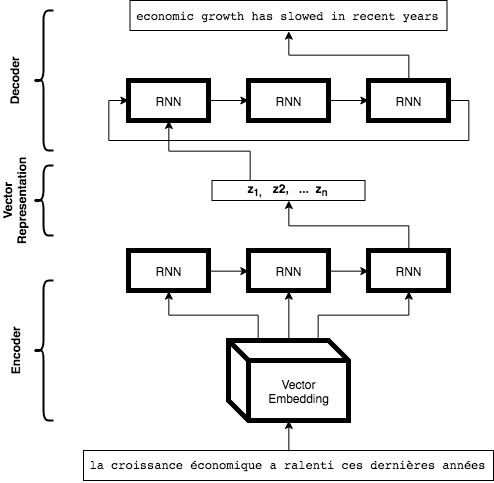
\includegraphics[width=.65\linewidth]{encoder_decoder_trans}
  \label{fig:test1}
\end{minipage}%
\begin{minipage}{.5\textwidth}
  \centering
  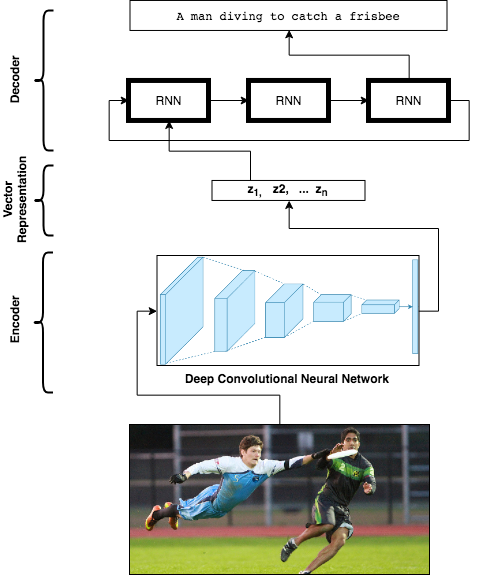
\includegraphics[width=.65\linewidth]{encoder_decoder_cnn}
  \label{fig:test2}
\end{minipage}
\caption{The encoder-decoder framework in neural machine translation models (left) and image captioning models (right). In machine translation applications, an input sequence is encoded by an RNN to a vector represention, before decoded to an output sequence. Analogously, a neural image captioning system uses a CNN to encode an input image before generating an output sequence.}
\end{figure*}

Traditional sequence prediction tasks - such as time series forecasting and language modeling - involve using a varying length sequence of inputs (whose ordering usually have a temporal interpretation), and predicting a single output (usually at the next time step). Neural networks are well equipped to solve this type of ``many-to-one" problem, as sequences of inputs may be coerced to a fixed number of time steps, so that the network does not need to account for varying length input or outputs.

Another class of sequence prediction task are those with varying length sequences as both inputs and outputs. These so-called ``many-to-many" or ``sequence-to-sequence" problems are more difficult than many-to-one problems, as the network must learn to produce predictions of varying lenghts.

An important example of a sequence-to-sequence problem is that of statistical machine translation (SMT). SMT models attempt to take in a sequence of words in one language, and output a sequence of words in another language, all while preserving the meaning of the input sequence and the coherence of the output sequence.


An approach which has proven effective in sequence-to-sequence prediction problems, including machine translation, is called the ``Encoder-Decoder" architecture. This architecture is comprised of two parts: the ``encoder" takes in a varying length input sequence, and encodes it into a fixed-length vector representation. The ``decoder" model decodes this vector representation into a varying-length sequence prediction. 

Cho et al. (2014) use this framework to build a SMT system which translates sequences from French to English. They use LSTM recurrent neural networks to encode input sequences, and LSTMs to decode the encoded representations to form the predictions. Cho et al. show that the encoded representations of input sequences preserve syntactic and semantic structure - thus, this representation is often referred to as a ``sequence embedding." Variants of encoder-decoder models have become the state of the art in machine translation; in fact, Google has adopted this approach in their Google Translate Service (Wu et al.; 2016).

Modern neural image captioning (NIC) systems, including those described in this paper, adopt this approach for the problem of image captioning. Image captioning is similar to machine translation in that the output is a varying length sequence of natural language, but differs in that the input is an image, rather than a sequence. Thus, instead of using RNN models such as LSTMs to encode the input, NIC systems typically use CNN models to form a vector representation from an image. Recurrent neural networks then use this representation to form an output sequence. Thus, NIC systems fall under the Encoder-Decoder framework, with CNNs acting as encoders and RNNs acting as decoders [figure 1]. 


The use of CNNs as encoders is justified by the success of CNNs in core computer vision tasks, such as image classification and segmentation. It is believed that CNNs succeed in these tasks becasue they can extract meaningful and complex features images effectively. Thus, just as LSTMs an encode the semantic and syntactic of an input sequence in SMT applications, it is believed that CNNs encode meaningful properties of an input image in NIC systems.

\subsection{Merge and Inject Models}

In a NIC system, CNN image features are combined with previously predicted tokens in a sequence to predict the next token in a sequence. The Encoder-Decoder framework includes a broad class of model architectures, and there are many ways to condition the sequence prediction on the image features, each of which uses the assigns a different role to the RNN component of a NIC system. 

In their paper \emph{What is the Role of Recurrent Neural Networks (RNNs) in an Image Caption Generator?}, 
Tanti et al. describe two important classes of NIC models that differ in their method of incorporating image features. 

The first, referred to as ``Condition-by-Inject" (or ``Inject" models for short), incorporate the CNN image features directly to the RNN component. Using both the image features and the previously predicted tokens to predict the next token of the sequence. This is ususally done by conditioning the internal state of the RNN cells with the image representation, or treating the image representation as the first `word' in the input sequence. The second method, called ``Condition-by-Merge" (or ``Merge" models for short), never incorporates the image features into the RNN model. Instead, the RNN is used to encode the linguistic features from previously predicted tokens, independent of the perceptual encoding formed by the CNN. Then, the linguistic and pereceptual encodings are merged to a single representation, from which the output prediction is made [figure 2]. 

\begin{figure*}[h]
\centering
\begin{minipage}{.5\textwidth}
  \centering
  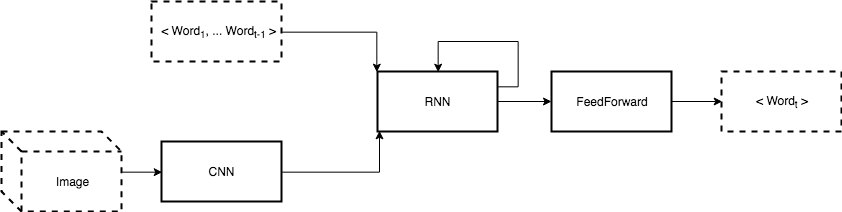
\includegraphics[width=.85\linewidth]{inject_scheme}
  \label{fig:test1}
\end{minipage}%
\begin{minipage}{.5\textwidth}
  \centering
  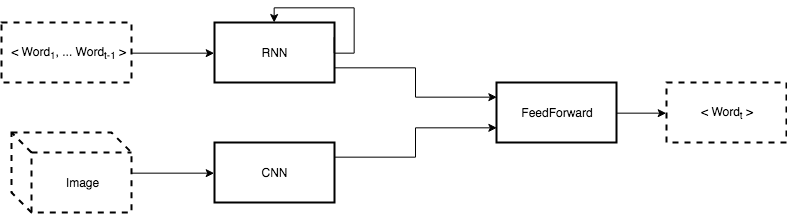
\includegraphics[width=.85\linewidth]{merge_scheme}
  \label{fig:test2}
\end{minipage}
\caption{A bare-bones diagram of the Inject architecture (left) and Merge architecture (right). The former conditions the RNN with both the image and linguistic features, and uses the RNN to generate new tokens. The uses the RNN to encode the previously predicted tokens into a vector representation, rather than to generate new tokens.}
\end{figure*}

The Inject and Merge architectures assign different conceptual roles to the RNN in a NIC system. In the Inject model, both perceptual and linguistic features are available to the RNN, which is responsible for generating the next predicted token. Thus, the RNN acts as a ``generator" in the Inject architecture. In contrast, the RNN has no access to the image freatures in the Merge architecture. Instead, the RNN encodes an input sequence into a fixed length vector represenation, and a later fully connected layer is responsible for generation of new tokens. Thus, in the Inject architectures, the RNN can be thought of as an encoder, rather than a generator. 

In the experiments described in section \textbf{ENTER SECTION}, I compare models using the Inject and Merge architectures. The idea that the choice of an Inject/Merge architecture dictates the `role' of the RNN in a NIC adds adds a new persepctive to these experiments. The relative efficacy of one architecture over another not only shows us which architecture is more appropriate for this taks, but provides insights into what settings RNNs best suited in general.  

\section{The Yelp Dataset}

Yelp maintains \href{https://www.yelp.com/dataset}{a public dataset} for the purposes of research and education. Part of this dataset is a collection of over 200,000 images uploaded by users, 100,807 with captions written by users upon uploading these images. This subset of images is what I used to train my image captioning system. 

Compared to standard benchmark datasets for image captioning, such as Flickr-8k and Flickr-30k, the Yelp dataset makes for a much more difficult task in training an effective NIC model.

Standard datasets typically have 4-8 training captions per image, which helps elucidate which words are related the an image's content, and which words are a result of more noisy phenomena, such as an author's writing style. 

More importantly, datasets such as Flickr-8k and Flickr-30k were collected by giving human subjects detailed instructions on how to form a training caption [figure 3]. In contrast Yelp users are given no guidance on what photos to upload to the site, nor how to write corresponding captions. The result is a dataset wit a much larger variablility in caption style, content and relevence to the task of image captioning. More severely, since the users are not given a common set of instructions on how to construct training captions, the task of modeling the image-caption relationship is not well defined. Figure 4 shows four images that make it difficult to train a NIC on the Yelp image dataset. 

\begin{figure}[]
\centering
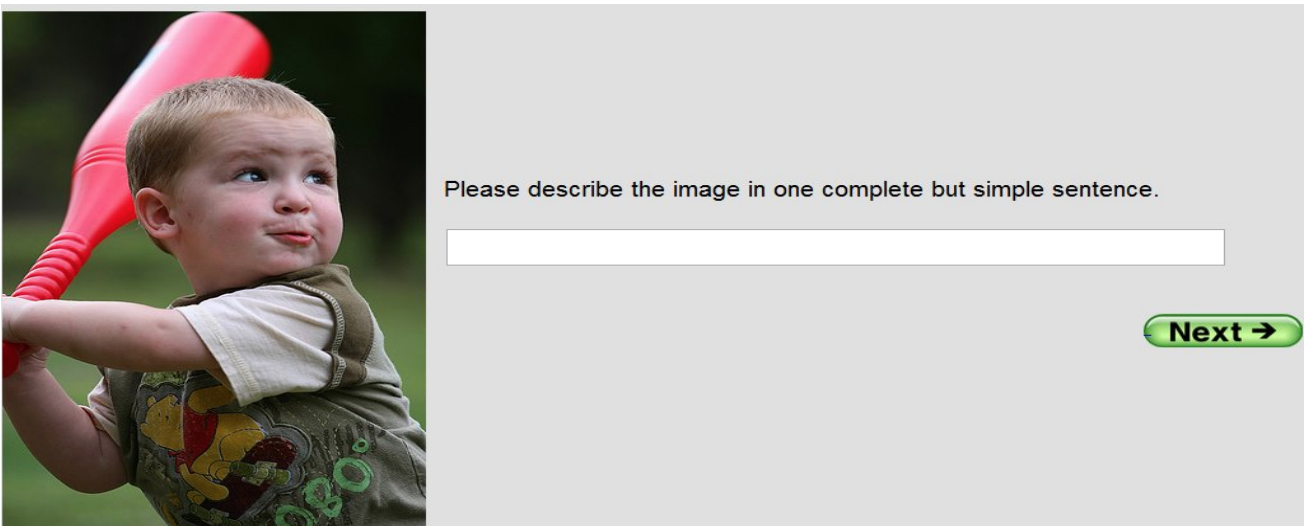
\includegraphics[width=1\linewidth]{boy}
\caption{Instructions presented to Amazon Turkers in the collection of the Flickr-8k dataset (Rashtchian et al., 2010). Image extracted directly from [7].}
\label{fig:test1}
\end{figure}


\begin{figure}[]
\centering
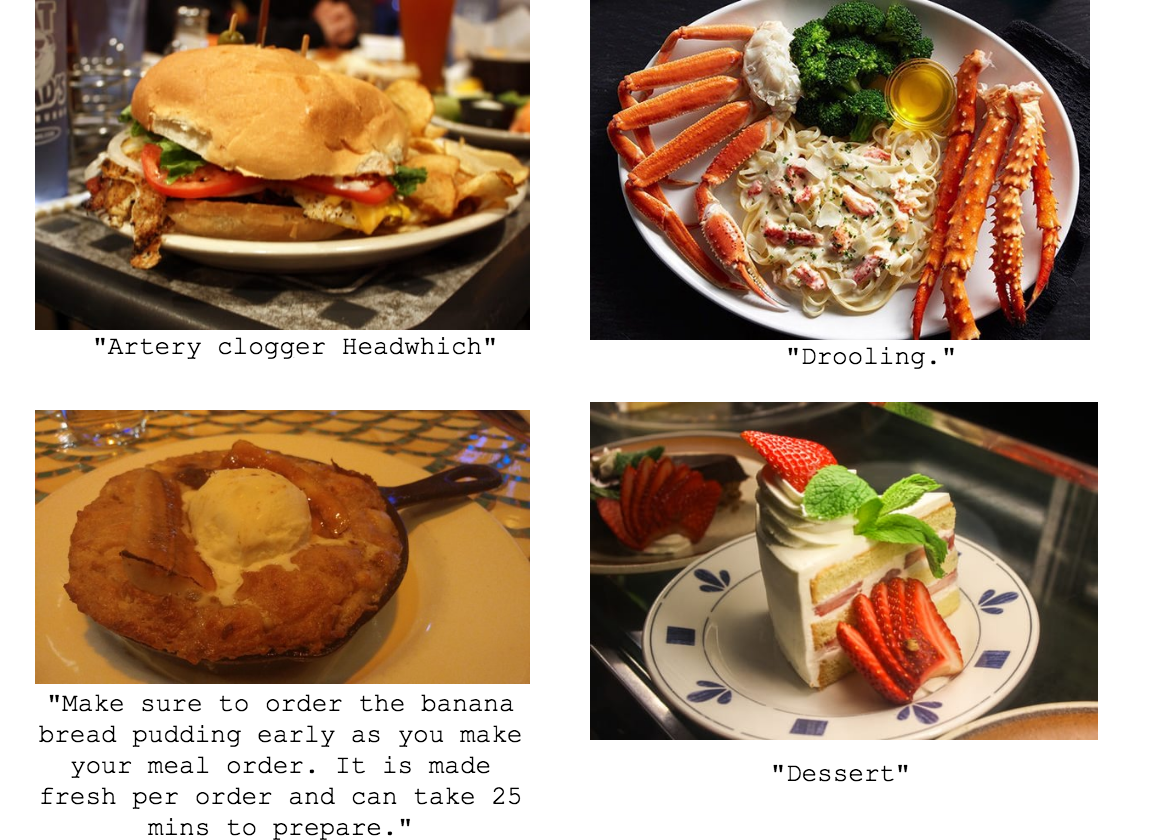
\includegraphics[width=1\linewidth]{im_quad}
\captionsetup{singlelinecheck=off}
\caption[list=off]{
Sample images from the Yelp image dataset, chosen to exemplify the varying sources of noise in the dataset.
\begin{itemize}
\item \emph{Top-left:} Rarely encountered noun-phrases such as `Artery clogger' and apocryphal words like `Headwhich' make it difficult to identify words tied to an image's content.
\item \emph{Top-right:} Captions which are unrelated to the image content.
\item \emph{bottom-left:} Wordy captions, which are likely to have content that is particular to an image, and does not generalize to images with similar content.
\item \emph{bottom-right:} Over simplified captions. This training example may cause a neural network to learn a link between the features of strawberry shortcake to the word \emph{dessert}, which describes a much larger class of dishes.
\end{itemize}
}
\end{figure}

It's clear that for a NIC to perform well on the Yelp dataset, one would have to invest considerable effort in structuring and cleaning the training data. As I only did minimal preprocessing (see section \textbf{INSERT PREPROCESSING SECTION}, I do not expect my system to generalize well. Instead, my goal is to study the practical challenges of building an image captioning system on `real-life' data. Perhaps the most pertinent challenge is collecting structured data which is designed for the task.

\section{METHODOLOGY}

In this section, I describe the preprocessing and feature extraction steps I took to prepare the Yelp dataset for training. I then outline the different model architectures I tested, and a custom scheme for generating caption from unseen images using these models. 

\subsection{Extracting Image Embeddings}

A NIC system must incorporate features extracted from both an input image and a partial caption \footnote{Initially, the `partial caption' is a special token that signifies the beginning of the predicted sequence, \texttt{<startseq>}. Then, one predicts the next word of the sequence and feeds it back to the network, until the token \texttt{<endseq>} is predicted by the network, which marks the end of the predicted sequence.} in order to predict the next word of the caption. This requires that one compress an input image into a fixed-length vector which encodes the visual features of the image - thus forming a sort of \emph{image embedding.}

One approach to doing so is to construct a model architecture in which input images pass through many layers - responsible for extracting informative features from the images - before incorporating these image features with the rest of the NIC model - and then training the entire model using back-propogation.  

The problem with this approach is that powerful neural networks that prove effective in various computer vision tasks often have many millions of parameters. Thus, a NIC that is trained to extract image features from scratch would likely be very deep and have many parameters\footnote{This argument uses the intuition that networks that achieve state of the art performance in classic tasks like image classification do a good job of extracting interesting features from images. Therefore, a network trained to form powerful image embeddings from scratch will likely also need to have many parameters.}, which leads to slow training, and a propensity to overfit.

\begin{figure*}[ht]
\centering
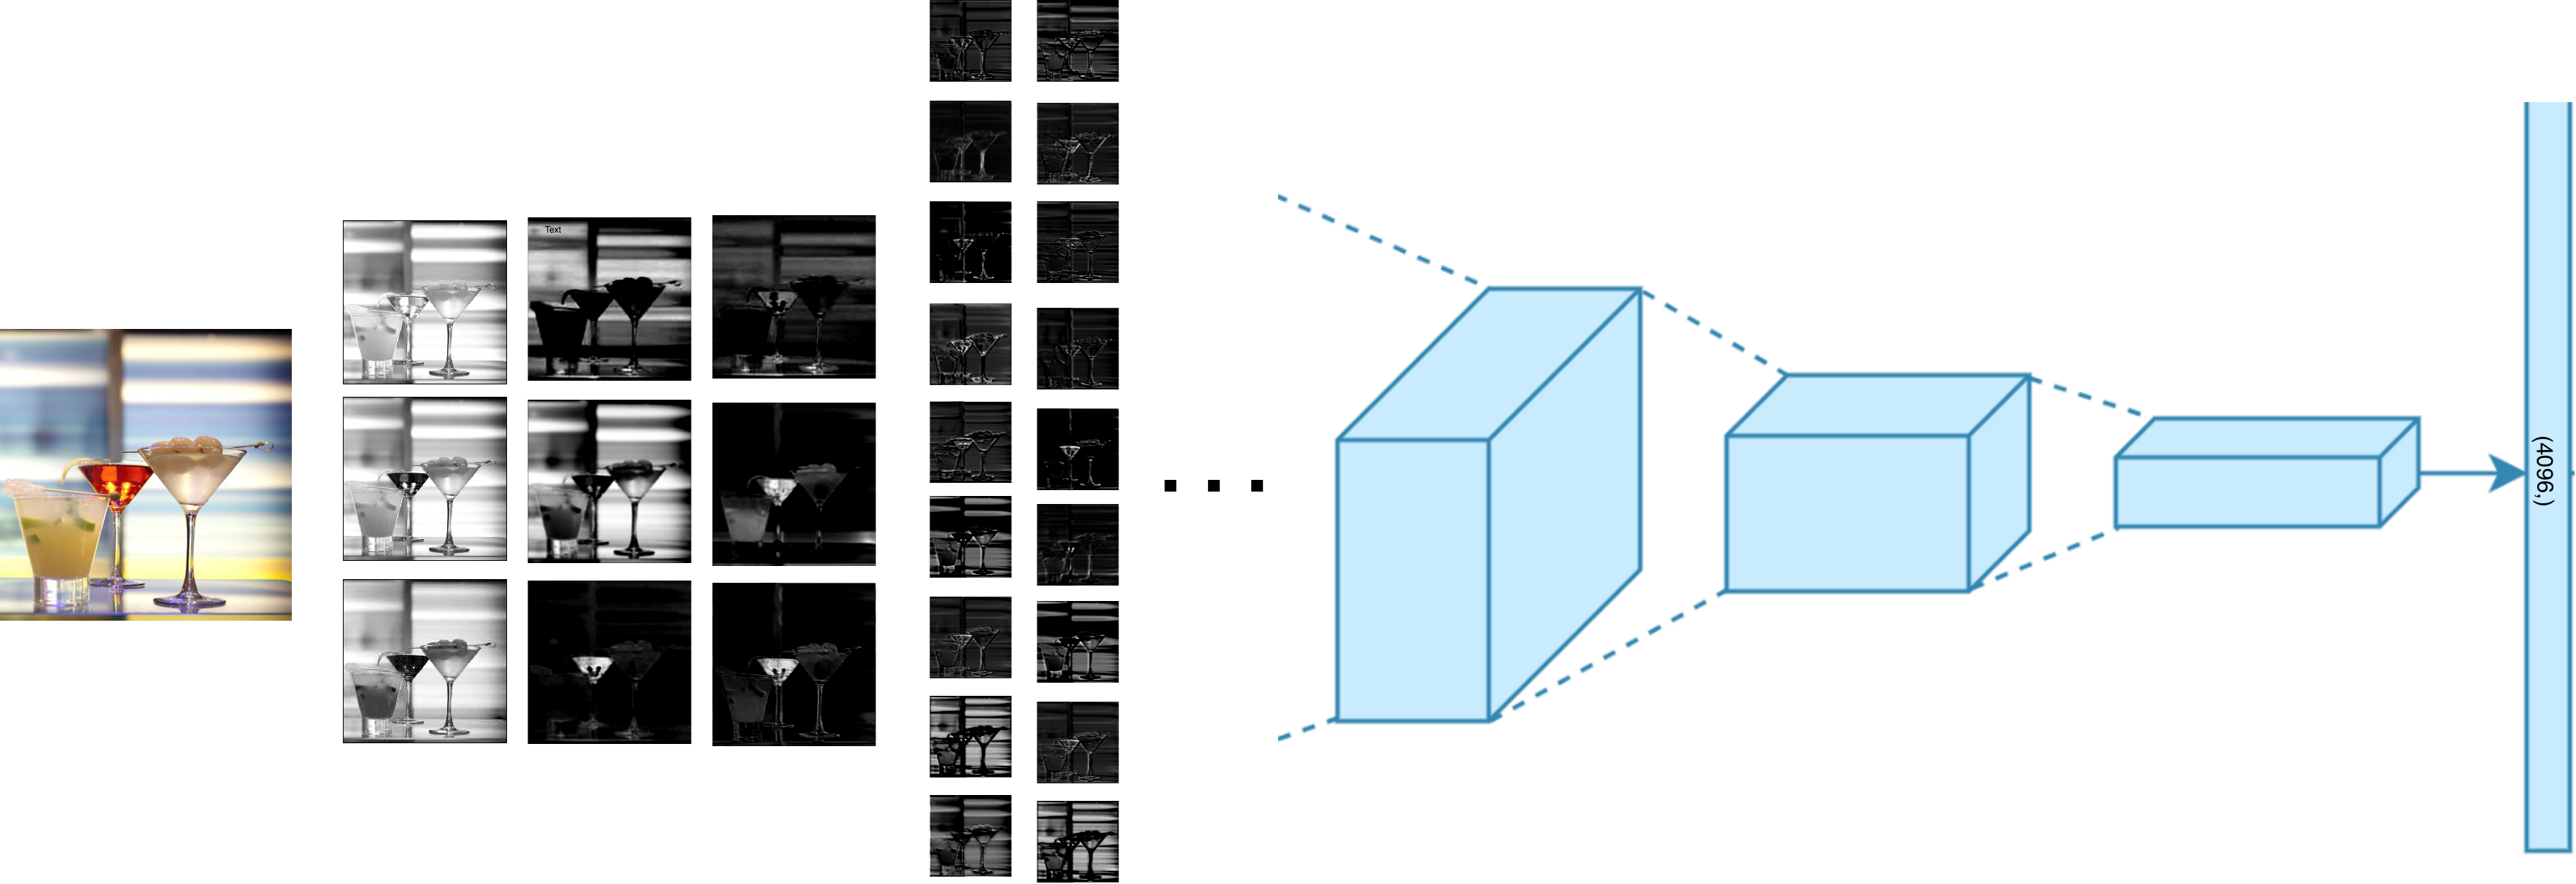
\includegraphics[width=1\linewidth]{cnn_features}
\caption{Vector representations of images, or ``image embeddings", are created by saving an intermediate activation of the VGG16 network, which is capable of detecting rich perceptual features, such as edges, blur and hue. These embeddings, combined with linguistic features, are used to generate captions for input images. Thus, the abridged VGG16 network may be thought of as the \emph{encoder} in the \emph{Encoder-Decoder} framework.}
\label{fig:test1}
\end{figure*}

Instead, to create image embeddings for each of the training images, I utilized the pre-trained weights of the VGG16 network (Simonyan \& Zisserman; 2014), available in the \code{keras} deep learning library (Chollet et al.; 2015). This network, with 138,357,544 parameters and trained on over 1.3 million images from the ImageNet dataset (Russakovsky et al.; 2015), secured the first and the second places in the ImageNet ILSVRC-2014 localisation and classification competitions, respectively. Thus, it is reasonable to assume that this network is capable of extracting complex feautres from diverse images. 

The last 3 layers of the VGG16 architecuture are fully connected layers, with dimensions $4096$, $4096$ and $1000$, respectively. To generate an image embedding for each image in the Yelp dataset, I first removed the last two fully connected layers from VGG16, and used the predictions of this abridged model as  the image embeddings [figure 5]. I justification for dropping the last two layers of VGG16 is that while shallow layers of the network are responsible for extracting revealing features, the final layers are specialized for the task they were trained for - namely ImageNet classification. Thus, omitting the final two layers allows me to encode each image as a $4,096$ dimensional vector which is both informative and generalizes to the image captioning task.


\subsection{Caption Text Preprocessing}

A widespread challenge in Natural Language Processsing (NLP) tasks is that corpus vocabularies are very sparse - meaning that few words occur many times, any many words occur few times. Empirical studies repeatedly show that the frequency of a word in a corpus is inversely proportional to its frequency rank -  a result commonly referred to as \emph{Zipf's Law} (Wyllys, R; 1981). Sparse vocabularies lead to models with many parameters, and makes it harder to generalize patterns learned during training. 

Thus, I performed a cursory clense of the captions provided in the Yelp dataset, with goal of reducing vocabulary size. This clense is by no means thorough, and is likely the bottleneck in my final captioning system. 

The steps I took - in order - are:
\begin{itemize}
\item Lowercase all characters.
\item Remove newline characters.
\item Replace the character \texttt{\&} with the word \texttt{and}. This is so the system will identify phrases like \texttt{sweet \& spicy} and \texttt{sweet and spicy} to be identical.
\item Convert strings which match a simple regex pattern of a website domain\footnote{The regex pattern used to detect webite domains is \texttt{[a-z\textbackslash:\textbackslash/\textbackslash.0-9]+\textbackslash.(org|com|net)}, using the python \texttt{re} library.} to the token \texttt{website}. This is because two images are in the Yelp dataset are unlikely to refer to the same website domain, leading to tokens of low frequency and a larger vocabulary.
\item For the same reasons, I replaced all tokens with numeric characthers with the token \texttt{num}.
\item Using the python \code{unidecode} library, I re-encoded all characters to ascii characters. This way, phrases with/without accents like \textit{gruyère soufflé} and \textit{gruyere souffle} are consolidated to the same tokens. The \code{unidecode} library also implements functions for transliterating tokens from forign languages to english characters, further reducing vocabulary size.
\item Remove all remaining punctuation.
\item Prepent all captions with the token \texttt{<startseq>}, and postpend with the token \texttt{<endseq>}, to mark the beginning and end of each caption.
\end{itemize}
After these steps, the processed captions contain 30,012 unique terms. 

\subsection{Formatting Data for Training}

Section 3.A discusses how one can conceptually fit the image captioning task into the probabilistic framework. Equation (2) shows that under mild assumptions, the probability of a caption being correct, given an image, can be decomposed into the probability of each token given the previous tokens and the image: 

\begin{equation*}
\log P(S_1, ... S_k | I; \theta) = \sum_{t = 1}^k{\log P(S_t|S_1 ... S_{t-1}, I; \theta)}
\end{equation*}

Typically, NIC systems model $P(S_t|S_1 ... S_{t-1}, I; \theta)$ with a recurrent neural network (RNN) sub-architecture. That is, the RNN is responsible for predicting the next token, given the previous tokens in the caption and the image; this way, the RNN plays the role of a language model. 

Inspired by (2), I reformat the training captions to be compatible with a language modeling task. First I extract an image embedding for each image in the dataset (section 5.A), and preprocess the text of the corresponding caption (section 5.B). Then, for each embedding/caption pair, I create a new training example for each token in the caption, where each token plays the role of the response, and the  covariates\footnote{\textit{Covariates}, as in the features which are trained upon. Also referred to as \textit{independend variables} or \textit{predictors}, and typically denoted as $\mathbb{X}$ in the statistics literature.} are the tokens that occur previously in the original caption, as well as a copy of the corresponding image embedding [figure 6].

\begin{figure}[H]
\centering
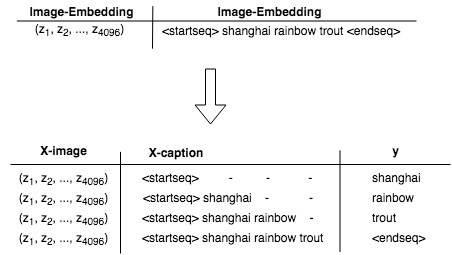
\includegraphics[width=1\linewidth]{caption_expand}
\caption{An example of how an image-embedding/caption pair is reformatted to suit a language modeling task. Each token (except for the first \texttt{<startseq>} token is treated as a response, where the covariates are the previous tokens in the sequence, and a copy of the image embedding.}
\label{fig:test1}
\end{figure}

Captions who exceed 15 tokens in length are truncated to 15 tokens. Captions that are shorter than 15 tokens are padded by a special \texttt{null} token. This way, all captions have a uniform length of 15 tokens.

After performing this expansion, the original 100,807 images with captions become 675,289 image-embedding/sub-caption pairs. When splitting the dataset into training/validation splits (section 6), I split the data \textit{before} performing the expansion detailed above. This is to ensure that the models are trained on complete captions.

\subsection{Model Architectures}


\begin{figure*}[h]
\centering
\begin{minipage}{.5\textwidth}
  \centering
  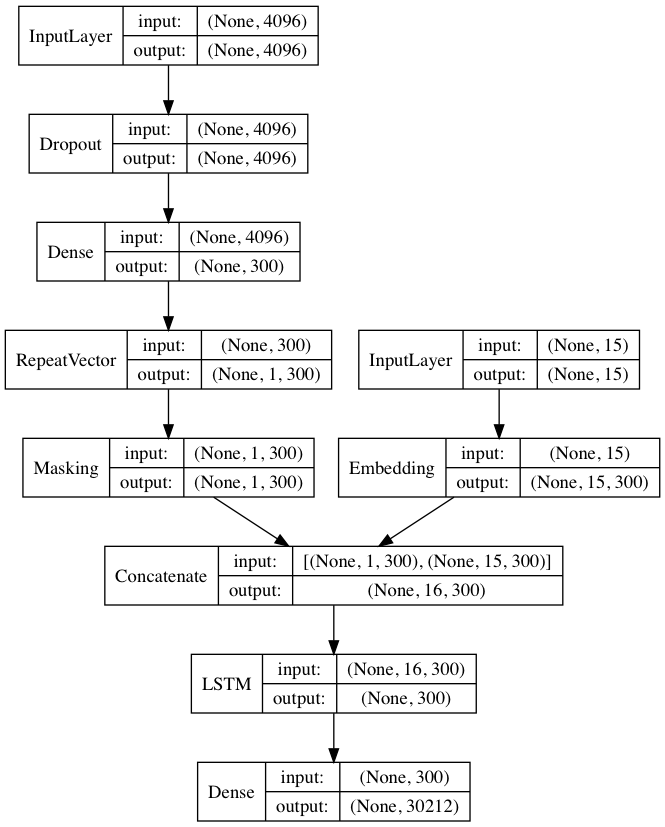
\includegraphics[width=.8\linewidth]{inject}
  \label{fig:test1}
\end{minipage}%
\begin{minipage}{.5\textwidth}
  \centering
  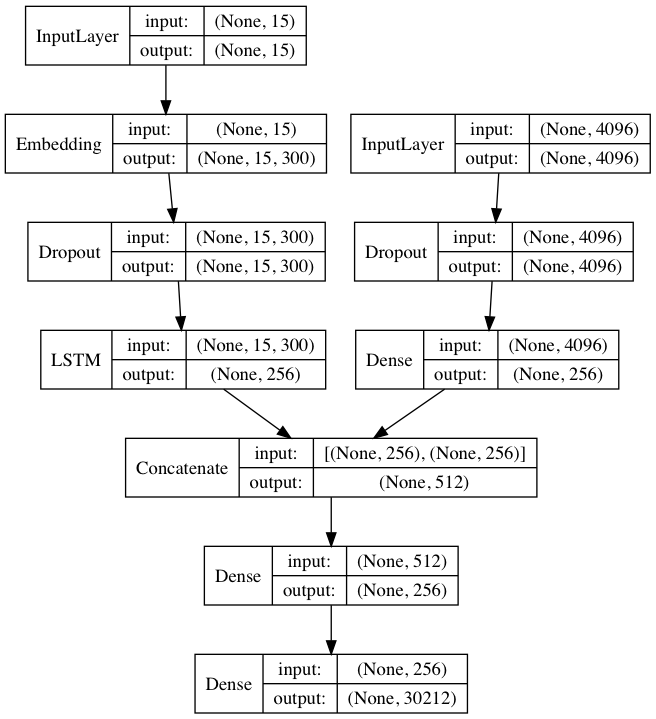
\includegraphics[width=.8\linewidth]{merge}
  \label{fig:test2}
\end{minipage}
\caption{Inject model (left) and merge-concat models (right). In the inject model, image features are treated as the first ``word" in the caption, then passed to the LSTM cell. In the merge-concat model, image and caption features are processed seperately, concatenated, then passed to a dense layer to form predictions. \\
The merge-add layer (not shown above) differs from the merge-concat model only in that image and caption features are \textit{added} instead of \textit{concatenated}. \\
Layer names above refer to \href{https://keras.io/layers/about-keras-layers/}{\texttt{keras} layer classes}.}
\end{figure*}

In this project, I experiment with three model architectures - two \textit{merge models} and one \textit{inject model}, in the language defined in section 3.C. See figure 7 for architecture details.

For all three models, the inputs are the same. Each training example is comprised of two input vectors - one for the image embeddings of dimension $(4096,)$, and an integer encoding of the input caption of dimension $(15,)$. The caption vectors are then passed to an embedding layer, where each token is represented as a 300 dimensional word embedding. I used pre-trained Word2Vec embeddings (Mikolov et al.; 2013), trained on the Google News corpus\footnote{Embeddings I used can be downloaded \href{https://github.com/mmihaltz/word2vec-GoogleNews-vectors}{here}.}. I configured these embedding weights to be fixed (non-trainable) in all three models. 

For the inject model, image embeddings are fed to a dense\footnote{Dense layers are fully connected layers.} layer of output dimension 300. The activation of this layer is then prependended to the word embeddings from the caption input, to form a volume of dimension $(16,300)$, which is then fed to an LSTM layer, with a hidden state of 300 dimensions. In other words, the image features are treated as the first ``word" in the sequence, before being processed by the RNN language model. The output of this LSTM is fed to a dense layer with a softmax activation to predict the next word in the sequence. I refer to this architecture as simply the ``inject model."

In both merge models, the captions - after being transformed to word embeddings - are passed to an LSTM cell  with a hidden state of 256 dimensions. Image embeddings are passed to a dense layer of output dimension 256. 

The activation of this dense layer is combined with the output of the final LSTM cell, thought he way they are combined differs between the two merge models. In the first, the two activations are \textit{concatenated}, yielding a single 512 dimensional vector, which is fed to a dense layer to form predictions. This model is referred to as the \textit{``merge-concat"} model. In the second, the two activations are \textit{added}, yielding a vector of dimension 256, which is passed to a dense layer to form predictions. This model is referred to as the \textit{``merge-add"} model.

The justification for experimenting with both the merge-concat and merge-add model is that the final dense layer of the merge-concat model has many parameters, as a 512 dimensional layer is fully connected to the final 30012 dimensional layer. The merge-add model halves the number of parameters in the final weight matrix, as a 256 dimensional layer is fully connected to the final 30012 dimensional layer.


\subsection{Inference as Beam Search}

The models detailed in section 5.D each take in two vectors as input - an image generated by passing an image through the VGG16 network, and the integer representation of a (partial) caption. The output of the models is a 30012 dimensional vector - where each element represents the predicted probability of a certain word appearing next in the caption. 

Given this setup, it is not trivial how to generate a new caption for an image previously unseen by the network, as partial captions are not availble during the inference stage. 

A naive method for generating new captions is \textbf{greedy selection}. Starting with an image features and a caption with only the start token \texttt{<startseq>}, one repeatedly uses a trained model to predict the probability of each word being next in the caption. Then, the word with the highest predicted probability is added to the caption. This process is repeated until the maximum sequence length is reached\footnote{In my models, I used a maximum sequence length of 15 tokens.}, or the special token \texttt{<endseq} is selected, marking the end of a sequence [algorithm 1].

\begin{algorithm*}[h]
\caption{Inference: Greedy Selection}\label{greedy-sampling}
\begin{algorithmic}[1]
\Procedure{GreedySelect(img-features, model)}{}
\State $\textit{caption} \gets \text{[}<startseq>\text{]}$
\Comment Initialize caption as start token.
\While {Length(caption) $<$ 15}
\Comment Repeat until generated caption is of maximum length.
\State $\textit{predictions} \gets \texttt{model.predict(img-features, caption)}$
\Comment Vector of predicted probabilities
\State $\textit{next-word} \gets \text{argmax(\textit{predictions})}$
\Comment Predicted next word is the one with the highest predicted probability.
\If {\textit{next-word} == \texttt{<endseq>}}
\State \textbf{break}
\Comment If end token is predicted, return caption as-is.
\Else
\State $\textit{cation} \gets \textit{cation}\text{.append(\textit{next-word})}$
\EndIf
\EndWhile
\Return \textit{caption}
\EndProcedure
\end{algorithmic}
\end{algorithm*}


\begin{algorithm*}[h]
\caption{Inference: Beam Search}\label{beam-search}
\begin{algorithmic}[1]
\Procedure{BeamSearch(img-features, model, $\beta$,$\kappa$, $\alpha$)}{}
\State $\textit{population} \gets \text{[}<startseq>\text{]}$
\Comment Initialize population as a single `starter' caption.
\State $i \gets 0$
\Comment Iteration Number
\For{$ i < 15 $}
\For{\text{each candidate caption } $S \in$ \textit{population}}
\If{Last token in candidate == \texttt{<endseq>}}
\State \textbf{break}
\EndIf
\State $\textit{predictions} \gets \texttt{model.predict(img-features, caption)}$
\Comment Vector of predicted probabilities
\State Add top $\kappa$ predicted words to caption to create $\kappa$ new candidates
\EndFor
\State Truncate poopulate top $\beta$ candidates, according to quality metric.
\State $i \gets i + 1$
\EndFor
\Return \textit{population}
\EndProcedure
\end{algorithmic}
\end{algorithm*}

In each iteration, greedy selection selects the word it finds most probable and adds it to the generated caption. It does not allow for adding words that may be ``suboptimal" at a given iteration, but then enables the model to make a prediction it is very confident of in a later iteration. Since our goal is to generate a sequence of tokens $\textbf{S}$ which well approximates the \textit{joint} probability of each of the tokens, $\textbf{S}^* = \argmax_{\textbf{S}}{P(S_1, S_2, ..., S_k|I)}$, it seems that this scheme is too rigid. 

A more flexible method of inference is \textbf{Beam Search}. Instead building up a single caption as greedy selection does, one maintains $\beta$ candidate solutions at all times, where $\beta$ is called the \textit{beam width.} The set of candidate solutions is often refered to as the \textit{population} of candidates. At each iteration, each candidate solution in the population is expanded into $\kappa$ candidates by adding the words with the top $\kappa$ predicted probabilities to the candidate, where $\kappa$ is called the \textit{neighborhood size.} After each candidate in the population is expanded into $\kappa$ new candidates, only the top $\beta$ candidates maintained (according to some metric of candidate quality), and move on the next iteration. 

The metric of candidate solution quality is yet to be defined. Previous work uses standard metrics designed for machine translation and image captioning tasks, such as BLEU (Xu et al.; 2015) and the MSCOCO evaluation code\footnote{https://github.com/tylin/coco-caption} (Tanti et al.; 2017). 

In this work, I define a custom quality metric inspired by personal model of what a ``good" predicted caption looks like. A good prediction should should be descriptive, and be relevant to an image's content. It should also be succinct, and avoid adding predicted tokens if the model is not ``confident" in these predictions. 

The quality metric is calculated as follows: for each candidate caption $S \equiv (S_1, S_2, ... S_k)$, keep track of the probabilities of each token $\Omega_S = (\omega_1, \omega_2, ... \omega_k)$\footnote{In this notation, $\omega_t$ is the predicted probability of the token $S_t$.}, predicted by the model during earlier iterations of the beam search. Then, the quality score of the sequence $S$ is a weighted sum of the predicted probabilities $\Omega_S$, where the weight multiplied by $\omega_t$ is $\alpha^t$, for some $\alpha \leq 1$: 

\begin{equation}
\text{Score}\big ( (\omega_1, \omega_2, ... \omega_k) \big ) = \sum_{t = 1}^k \omega_t\cdot\alpha^t
\end{equation}

This measure rewards candidates whose tokens are predicted with high probability, but discounts later tokens due to the geometric decrease in weights, $\alpha^t$. Thus, $\alpha$ is a sort of regularization hyperparameter - small values of $\alpha$ leads to terse captions, while large values of $\alpha$ leads to captions at or near the maximum token length [figure 8].  

\begin{figure}[h]
\centering
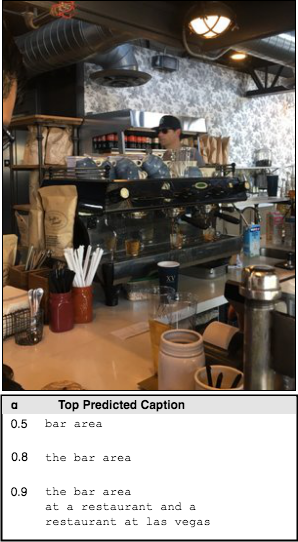
\includegraphics[width=.6\linewidth]{alpha_affect}
\caption{Top caption predictions using beam search and the inject model, for different values of $\alpha$. Small values of $\alpha$ lead to overly terse captions, while large values of $\alpha$ lead to wordy and repetitive captions.}
\label{fig:test1}
\end{figure}

Note that greedy selection is a special case of beam search, where $\beta = \kappa = \alpha = 1$.  


\bibliographystyle{IEEEtran}
\bibliography{\jobname}
\end{document}
